\vspace{-2mm}
\section{Programming Interface}
\label{sec:parser}
Spark SQL provides two programming interfaces, the SQL-like relational
query language and the DataFrame API \cite{sparksql}, so that users
can easily express their analytical queries and integrate with other
systems in the Spark ecosystem. \name extends both of the interfaces
to support spatial queries and analytics. We first discuss the
extensions made to the SQL query language in \name.


\begin{figure}[t!]
	\centering
	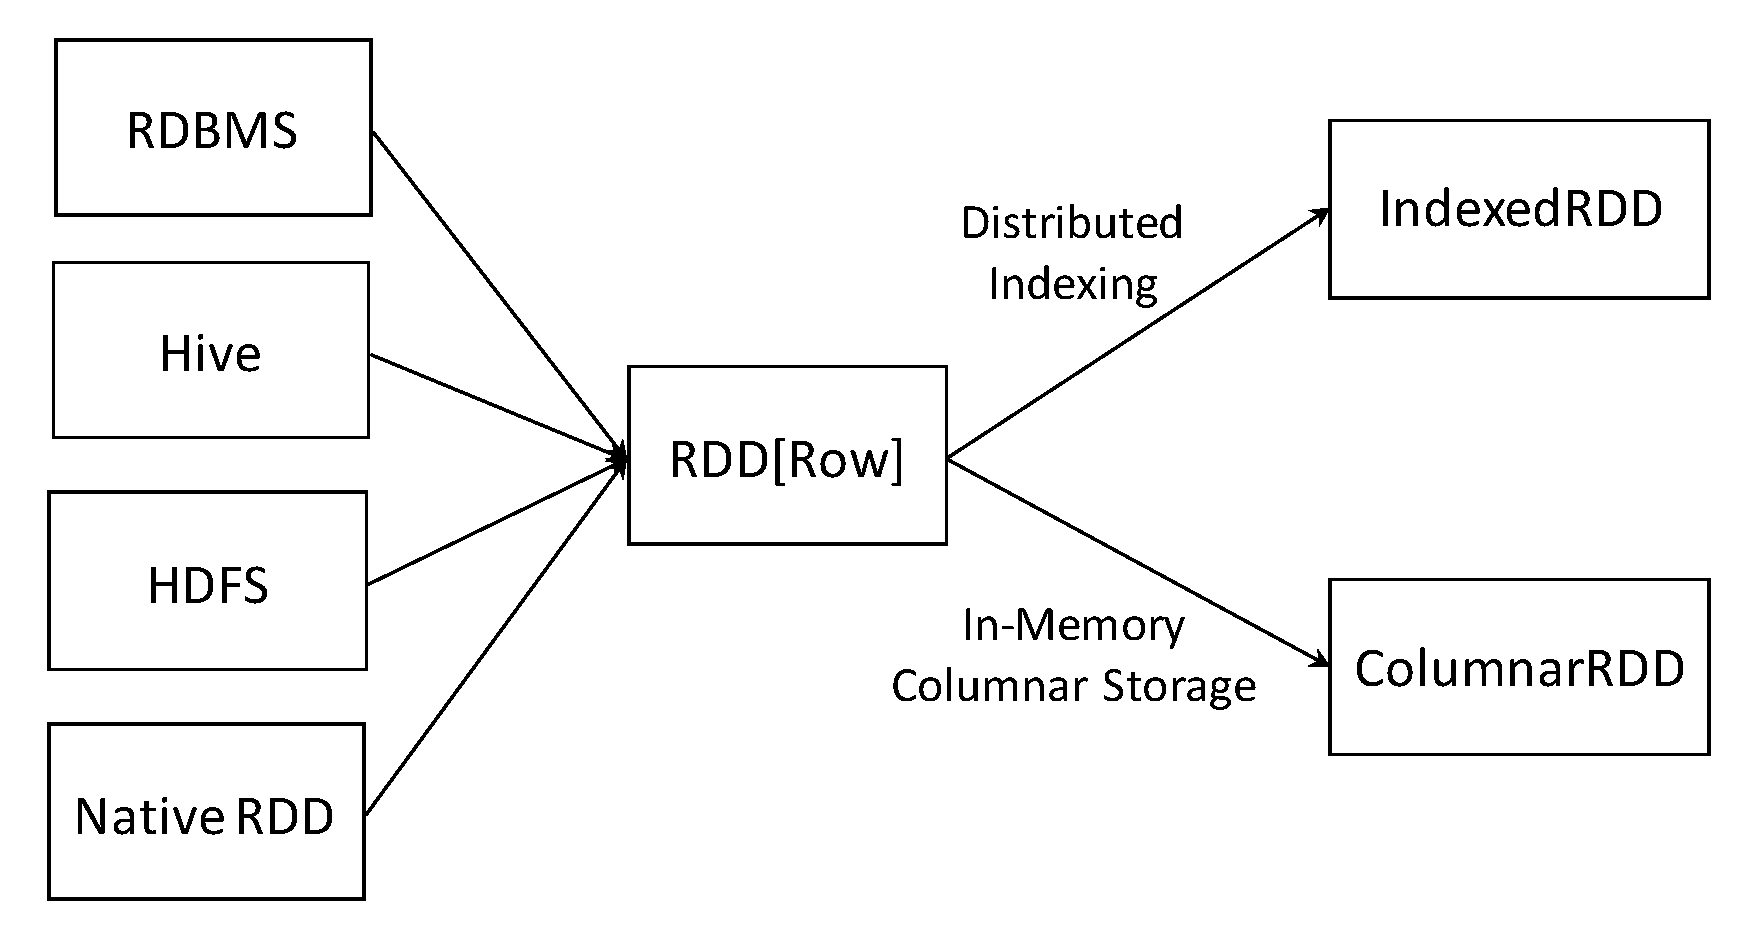
\includegraphics[width = 3.2in]{figs/storage}
	\vspace{-3mm}
	\caption{Data Representation in \name.}
	\label{fig:storage}
	\vspace{-3mm}
\end{figure}



\Paragraph{Points.} Users can express a multi-dimensional point with
the keyword \texttt{POINT}. Not only constants or attributes of
tables, but also arbitrary arithmetic expressions can be used as the
coordinates of points. For example, users can use \texttt{POINT(x + 2,
  y - 3, z * 2)} to express a three dimensional point with the first
coordinate being the addition of attribute \texttt{x}'s value and
constant 2. This offers a flexible way to express spatial points in
the SQL query language. In \name, we will calculate each expression
in the statement and wrap them as a point object for further processing.

\Paragraph{Spatial predicates.} \name adds several new predicates to
SQL to support spatial queries, such as \texttt{RANGE} for box range
queries, \texttt{CIRCLERANGE} for circle range queries with a radius,
and \texttt{KNN} for $k$ nearest neighbor queries. For instance, users
can ask for the 3-nearest neighbors of point $(4, 5)$ from table
\texttt{point1} as below:
\begin{lstlisting}[language=SQL]
SELECT * FROM point1
WHERE POINT(x, y) IN KNN(POINT(4, 5), 3).
\end{lstlisting}\vspace{-2mm}

And a box range query as below asks for all points from table
\texttt{point2} in the 2 dimensional rectangle defined by point
$(10, 5)$ (lower left corner) and $(15, 8)$ (top right corner):
\begin{lstlisting}[language=SQL]
SELECT * FROM point2
WHERE POINT(x, y) IN RANGE(POINT(10, 5), POINT(15, 8)).
\end{lstlisting}\vspace{-1mm}

\Paragraph{Spatial joins.} \name supports two types of spatial joins:
distance joins and $k$NN joins.  Users can express these spatial joins
in a $\theta$-join like manner. Specifically, a 10-nearest neighbor
join between two tables, \texttt{point1} and \texttt{point2}, can be
expressed as:
\begin{lstlisting}[language=SQL]
SELECT *
FROM point1 AS p1 KNN JOIN point2 AS p2
ON POINT(p2.x, p2.y) IN KNN(POINT(p1.x, p1.y), 10).
\end{lstlisting}\vspace{-2mm}

A distance join with a distance threshold $20$, between two tables
\texttt{point3} and \texttt{point4} in 3 dimensional space, is
expressed as:
\begin{lstlisting}[language=SQL]
SELECT *
FROM point3 AS p3 DISTANCE JOIN point4 AS p4
ON POINT(p4.x, p4.y, p4.z) IN CIRCLERANGE(POINT(p3.x, p3.y, p3.z), 20).
\end{lstlisting}\vspace{-2mm}



\Paragraph{Indexing command.} Users can manipulate indexes in \name
easily with indexing commands introduced by \name. For example, users
can build an R-Tree index called \texttt{pointIndex} on attributes
\texttt{x}, \texttt{y}, and \texttt{z} for table \texttt{sensor} using
command:
\begin{lstlisting}[language=SQL]
CREATE INDEX pointIndex ON sensor(x, y, z) USE RTREE.
\end{lstlisting}\vspace{-2mm}

\Paragraph{Complex queries.} Note that \name has kept the support for
all grammars (including UDFs and UDTs) supported by Spark SQL. As a
result, we can express complex spatial queries in a single SQL
statement. For example, we can count the number of restaurants near
(say within distance 10) a POI for a set of POIs, and sort
locations by the counts, with the following query:
\begin{lstlisting}[language=SQL]
SELECT q.id, count(*) AS c
FROM pois AS q DISTANCE JOIN rests AS r
ON POINT(r.x, r.y) IN CIRCLERANGE(POINT(q.x, q.y), 10.0)
GROUP BY q.id
ORDER BY c.
\end{lstlisting}\vspace{-2mm}

\Paragraph{DataFrame support.} Besides SQL, user can also perform
spatial operations on DataFrames using a domain-specific language
(DSL) similar to R data frames. \name's DataFrame API supports all
spatial operations extended to the SQL query language described
above. Naturally, all new operations are also compatible with the
exiting ones from R and Spark SQL, which provides the same level
flexibility as \name's SQL does. For instance, we can also the last
SQL query above in the following scala code:
%including range queries (\texttt{range}), $k$ nearest neighbors (\texttt{knn}), distance joins (\texttt{distanceJoin}) and $k$NN joins (\texttt{knnJoin}).
\begin{lstlisting}
pois.
  .distanceJoin(rests, Point(pois("x"), pois("y")),
                       Point(rest("x"), rest("y")), 10.0)
  .groupBy(pois("id"))
  .agg(count("*").as("c")).sort("c").show().
\end{lstlisting}

%%% Local Variables:
%%% mode: latex
%%% TeX-master: "paper"
%%% End:
